\documentclass{beamer}
\usefonttheme[onlymath]{serif}
\usepackage{amsmath}
\usepackage{amsfonts}
\usepackage[export]{adjustbox}
\usepackage[utf8]{inputenc}
\usepackage{tikz} 
\usepackage{bm}
\usetikzlibrary{bayesnet}

% definitions
\def\H{\mathcal{H}}
\def\X{\mathbf{X}}
\def\w{\mathbf{w}}
\def\W{\mathbf{W}}
\def\const{\mathrm{const}}
\def\Var{\mathrm{Var}}
\def\tr{\mathrm{tr}}
\def\T{\top}
\def\U{\mathbf{U}}
\def\S{\mathbf{S}}
\def\V{\mathbf{V}}
\def\N{\mathcal{N}}
\def\E{\mathbb{E}}
\newcommand{\argmin}{\mathop{\mathrm{argmin}}}
\newcommand{\argmax}{\mathop{\mathrm{argmax}}}
\newcommand{\minimize}{\mathop{\mathrm{minimize}}}
\newcommand{\maximize}{\mathop{\mathrm{maximize}}}
\newcommand{\st}{\mathop{\mathrm{subject\,\,to}}}
\newcommand{\mat}[1]{\begin{bmatrix}#1\end{bmatrix}}

%Information to be included in the title page:
\usecolortheme{seahorse}
\title{Causality}
\author{Kangcheng Hou}
\institute{Zhejiang University}
\date{\today}

% reference: 
% http://www.inference.vc/untitled/

    
\begin{document}
    
\frame{\titlepage}
\begin{frame}{Difference between $p(y | x)$ and $p(y | \text{do}(x))$}
In supervised learning setting, we are interested in $p(y | x)$. In causal inference, we are interested in $p(y | \text{do}(x))$. An example is consider $x$ as the temperature on thermometer, $y$ as the real temperature. $p(y|x)$ will be a unimodal distribution around $x$ because of the measure noise. And $p(y | \text{do}(x))$ will not be influenced by the value of $x$. Because $y$ is not determined by $x$. This is the \textbf{difference} between observational and interventional conditionals. 


\end{frame}

\begin{frame}{What is $p(y | \text{do}(x))$?}
We can imagine there is an underlying distribution $(x,y)$. $p(y | \text{do}(x))$ actually modifies the generating process of data. So it is no longer the original natural data generating process. Although it does not describe the data generation process, this distribution is still very interesting to us.

$p(y | \text{do}(x))$ is not some mysterious thing. We can perform \textbf{randomized controlled trials} with the data where we manipulate $x$ manually and use supervised learning method to estimate this. But the reality is that we can't do such \textbf{randomized controlled trials} at our free will. Even if we can't do experiments, the distribution $p(y | \text{do}(x))$ still exists. It turns out that $p(y | \text{do}(x))$ and $p(y | x)$ are connected.

\end{frame}

\begin{frame}
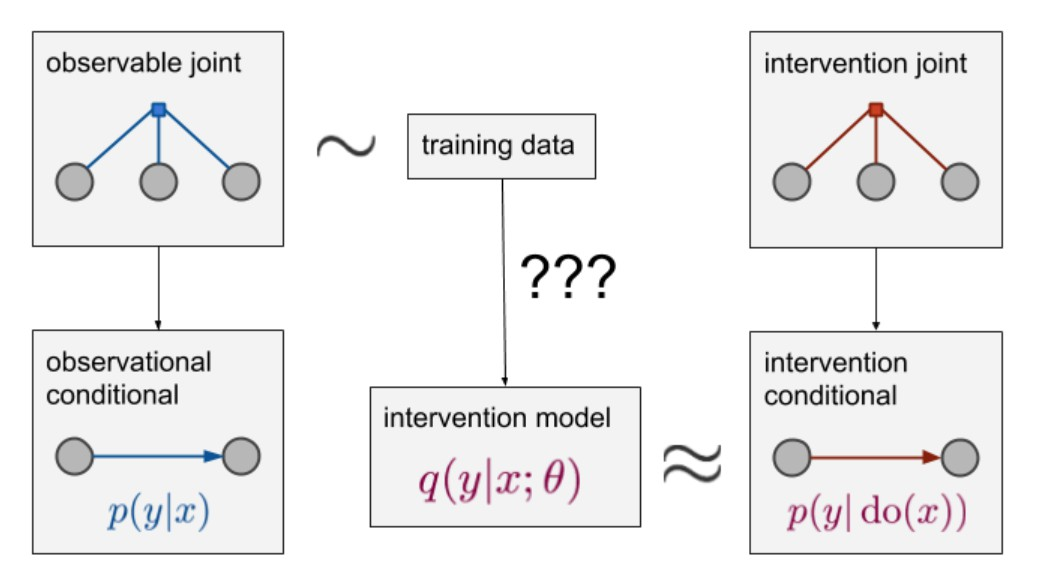
\includegraphics[width=0.8\textwidth]{./img/link.jpg}

$p(y | \text{do}(x))$ is defined on the same domain as $p(y | x)$ but is a different distribution. If we have data points sampled from $p(y | \text{do}(x))$, the problem will be easier via supervised learning (a.k.a curve fitting). It turns out that if we assume some causal structure of the problem, we can get something about $p(y | \text{do}(x))$ from samples of $p(y | x)$.
\end{frame}

\begin{frame}{Inference about the causal structure}
Information causal relationships is not captured in the joint distribution alone. 

\end{frame}
\end{document}